% !TeX encoding = UTF-8
% !TeX spellcheck = it_IT
% !TeX root = main.tex

\section{Descrizione dei tag}

\subsection{Persone e ruoli}
Uno dei principali obiettivi del sistema è l'individuazione di persone e dei ruoli che esse svolgono nella procedura fallimentare, ovviamente basandoci su ciò che troviamo all'interno dei moduli di richiesta.

Nei vari modelli di richiesta abbiamo individuato principalmente tre entità da poter ritrovare: \fbox{giudice}, \fbox{soggetto} e \fbox{curatore}.
Il primo è spesso individuato ad inizio documento, nell'intestazione, come destinatario della richiesta.
Il soggetto della richiesta è colui che la produce e la firma, spesso preceduto dalla parola ``sottoscritto'' e dalla sua presenza in calce.

Di seguito lo schema delle dipendenze dei tag per le persone e i loro ruoli.

\begin{figure}[H]
\centering
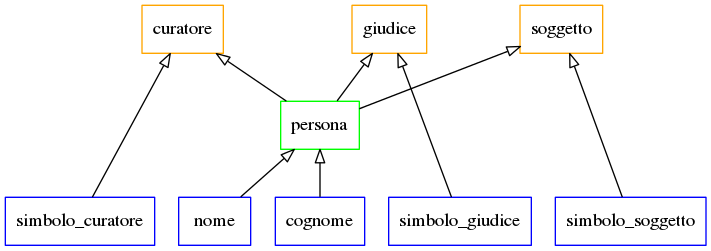
\includegraphics[width=.7\textwidth]{img/persona.png}
\label{fig:persona}
\caption[Dipendenze tra i tag - Persone]{Schema delle dipendenze dei tag per le persone e i loro ruoli}
\end{figure}

Nell'operazione di tagging vengono ricercati i simboli peculiari delle tre entità, ossia i token che contengono parole chiave da noi precedentemente individuate.
Il tag \verb|parola(giudice)|, ad esempio, introdurrà un \fbox{simbolo\_giudice}. \emph{Sottoscritto} o \emph{sottoscritta}, introdurranno un \fbox{simbolo\_soggetto} mentre \emph{curatore} determinerà un \fbox{simbolo\_curatore}.

Ciascuno di questi tre, associati ad un \verb|tag| \fbox{persona}, costituirà l'entità target che cercavamo in partenza.

Il tag persona merita un discorso a parte.
Il tag \fbox{persona} nasce dalla presenza di \fbox{nome} e \fbox{cognome} in entrambe le permutazioni.
Per questi ultimi 2 tag abbiamo effettuato una ricerca online di diversi database di nomi e cognomi italiani, fondendoli in un file Prolog \verb|persona_kb.pl|, consultato e utilizzato dal modulo \verb|persona|.

Abbiamo previsto la possibilità che ci siano nomi e cognomi composti. La legge italiana stabilisce un limite massimo di 3 nomi e 2 cognomi.
Le regole, di conseguenza, valuteranno come possibili nomi/cognomi sia le singole parole che corrispondono a voci del database, sia a parole concatenate (fino a 3/2), ciascuna delle quali è un possibile nome/cognome.

Ad esempio, prendendo in considerazione delle generalità abbastanza complesse come: ``Simone Addario Chieco'', il sistema ritroverà tanti possibili cognomi:

\begin{prologcode}
cognome('Simone').
cognome('Addario').
cognome('Chieco').
cognome('Simone Addario').
cognome('Addario Chieco').
\end{prologcode}

ma un solo nome

\begin{prologcode}
nome('Simone').
\end{prologcode}

L'unica persona identificata sarà, dunque, l'unica possibile, cioè con nome ``Simone'' e cognome ``Addario Chieco''.

In casi fortemente ambigui, però, come ad esempio ``Cataldo Roberto'' (entrambe le parole possono essere sia nomi o cognomi), il sistema non sarà in grado di disambiguare. Ritroverà la persona Cataldo/Roberto e la persona Roberto/Cataldo. Tuttavia, senza disporre di ulteriore conoscenza sulla persona, questo rimane un compito impossibile anche per l'essere umano.

\subsection{Richiesta economica}

Come descritto nella sezione \ref{sec:tipologiaIscrizione}, ci sono due tipi di tipologie: chirografaria e privilegiata.

Una valuta, invece, è rappresentata da un numero, intero o decimale, seguito o preceduto da un simbolo di valuta (per semplicità abbiamo preso in considerazione solo € e \$\footnote{Sono state prese in considerazione anche parole che potessero sostituire il simbolo. Per quanto riguarda il simbolo €, ad esempio, \emph{euro} ed \emph{eur}. Per il \$: \emph{dollaro}, \emph{dollari}, \emph{dollar}, \emph{USD}.})

Di seguito rappresentiamo lo schema delle dipendenze dei tag, per quanto concerne la richiesta economica.

\begin{figure}[H]
\centering
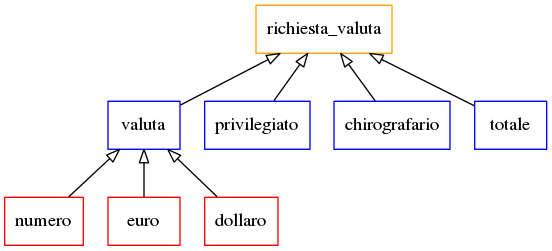
\includegraphics[width=.7\textwidth]{img/valuta.png}
\label{fig:valuta}
\caption[Dipendenze tra tag - Valute]{Schema delle dipendenze dei tag per le valute e le richieste economiche.}
\end{figure}

\subsection{Data}
Esistono numerosi modi per rappresentare una data (1/7/1988, 01-07-88, 1 luglio 1988, etc.).

Decomponendo il problema, una data è composta da un giorno, un mese e un anno.
Giorno e anno sono rappresentati esclusivamente con un numero mentre il mese può anche essere scritto col suo nome.

Il giorno è un numero intero compreso tra $1$ e $31$ (l'astrazione ottenuta dall'individuazione del tag numero ci permette di comprendere indistintamente la scrittura di $01$ e $1$).

Il mese può essere scritto come numero intero compreso tra $1$ (o $01$) e $12$ o col suo nome per intero (gennaio, febbraio), o ancora con l'abbreviazione del suo nome (gen, feb).

L'anno è un numero intero di 2 cifre compreso tra $00$ e $99$ e di 4 cifre compreso tra (per motivi inerenti al dominio) $1900$ e $2050$.

\subsection{Numero Pratica}
L'identificatore della pratica di fallimento, riportata in testa al documento, è composto da un numero intero, un separatore (\verb|/| o \verb|-|) e l'anno della pratica, ad esempio: \verb|10/2007|.

Utilizza i tag \fbox{numero}, \fbox{separatore\_data}, e \fbox{anno}.

\subsection{Numero Telefonico}
Nel tagging dei numeri telefonici abbiamo dovuto tenere in considerazione la presenza di numerose varianti.

Un numero di telefono può derivare da una sola concatenazione di cifre lunga 10 caratteri (3402158976) oppure essere composto da più gruppi separati da spazi (340 21 58 976) o da caratteri di separazione (340-215.8976). Per ognuno dei casi precedenti può essere presente o meno un prefisso internazionale che varia da 2 caratteri (+1 per USA e Canada) a 6 caratteri (001876 per la Giamaica).

Come per i cognomi e i nomi, è stato creato un file contenente tutti i prefissi (\verb|tel_kb.pl|) e sono state scritte numerose regole per individuare i diversi tipi di numeri telefonici.

\subsection{Mail}
Il tagging di un indirizzo mail avviene quando ci sono 3 token consecutivi e il secondo corrisponde al carattere ``@''.

\subsection{Comune}
Il tag comune deriva dal token o da una lista di token consecutivi che corrispondono ad uno dei comuni italiani. L'elenco dei comuni è stato trovato in rete e trasformato in fatti Prolog nel file \verb|comune_kb.pl|.

\subsection{Codice Fiscale}
Il codice fiscale è un tag semplice che necessita di tag precedenti. Si ottiene con un'analisi dei caratteri che compongono il token.

A partire da un token si genera un tag \fbox{codice\_fiscale} se esso è composto da una stringa lunga 16 caratteri, composta, nell'ordine, da 6 lettere, 2 numeri, 1 lettera, 2 numeri, 1 lettera, 3 numeri e 1 lettera.

Il codice Prolog scritto è il seguente:

\begin{prologcode}
check_cf(CF) :-
  atom(CF),
  atom_length(CF,16),
  atom_codes(CF,CFs),
  CFs=[C1,C2,C3,C4,C5,C6,C7,C8,C9,C10,C11,C12,C13,C14,C15,C16],
  ascii_char(C1),
  ascii_char(C2),
  ascii_char(C3),
  ascii_char(C4),
  ascii_char(C5),
  ascii_char(C6),
  ascii_number(C7),
  ascii_number(C8),
  ascii_char(C9),
  ascii_number(C10),
  ascii_number(C11),
  ascii_char(C12),
  ascii_number(C13),
  ascii_number(C14),
  ascii_number(C15),
  ascii_char(C16).
\end{prologcode}